\documentclass{report}
\usepackage[showframe=false]{geometry}
\usepackage{titlesec}
\usepackage{amsmath}
\usepackage{graphicx}

\pagenumbering{gobble}

\geometry{tmargin=60pt,bmargin=90pt,lmargin=90pt,
rmargin=90pt}

\titleformat{\chapter}{\normalfont\huge}{\thechapter.}{20pt}{\huge}
\titlespacing*{\chapter} {0pt}{0pt}{10pt}

\begin{document}

\chapter{Section 1}
\section{a.}

The vertebral column data was first read from the ARFF file, then split into classes for processing.

\begin{verbatim}
  library(foreign)
  vert <- read.arff("column_2C_weka.arff")
  vert_split <- split(vert, vert[,"class"])

  sapply(vert_split$Abnormal[0:6], mean)
  sapply(vert_split$Abnormal[0:6], median)
  sapply(vert_split$Abnormal[0:6], sd)
  sapply(vert_split$Normal[0:6], mean)
  sapply(vert_split$Normal[0:6], median)
  sapply(vert_split$Normal[0:6], sd)
\end{verbatim}

\subsection{Abnormal Data}

\begin{tabular}{l}
  mean \\
  \hskip 1.0cm\begin{tabular}{rrr}
    pelvic\_incidence & pelvic\_tilt & lumbar\_lordosis\_angle \\
    64.69256 & 19.79111 & 55.92537 \\
    sacral\_slope & pelvic\_radius & degree\_spondylolisthesis \\
    44.90145 & 115.07771 & 37.77771 \\
  \end{tabular} \\
  standard deviation \\
  \hskip 1.0cm\begin{tabular}{rrr}
    pelvic\_incidence & pelvic\_tilt & lumbar\_lordosis\_angle \\
    65.27489 & 18.79890 & 56.15000 \\
    sacral\_slope & pelvic\_radius & degree\_spondylolisthesis \\
    44.63960 & 115.65032 & 31.94652 \\
  \end{tabular} \\
  median \\
  \hskip 1.0cm\begin{tabular}{rrr}
    pelvic\_incidence & pelvic\_tilt & lumbar\_lordosis\_angle \\
    17.66213 & 10.51587 & 19.66947 \\
    sacral\_slope & pelvic\_radius & degree\_spondylolisthesis \\
    14.51556 & 14.09060 & 40.69674 \\
  \end{tabular}
\end{tabular}

\subsection{Normal Data}

\begin{tabular}{l}
  mean \\
  \hskip 1.0cm\begin{tabular}{rrr}
    pelvic\_incidence & pelvic\_tilt & lumbar\_lordosis\_angle \\
    51.685244 & 12.821414 & 43.542605 \\
    sacral\_slope & pelvic\_radius & degree\_spondylolisthesis \\
    38.863830 & 123.890834 & 2.186572 \\
  \end{tabular} \\
  standard deviation \\
  \hskip 1.0cm\begin{tabular}{rrr}
    pelvic\_incidence & pelvic\_tilt & lumbar\_lordosis\_angle \\
    50.12312 & 13.48243 & 42.63892 \\
    sacral\_slope & pelvic\_radius & degree\_spondylolisthesis \\
    37.05969 & 123.87433 & 1.15271 \\
  \end{tabular} \\
  median \\
  \hskip 1.0cm\begin{tabular}{rrr}
    pelvic\_incidence & pelvic\_tilt & lumbar\_lordosis\_angle \\
    12.368161 & 6.778503 & 12.361388 \\
    sacral\_slope & pelvic\_radius & degree\_spondylolisthesis \\
    9.624004 & 9.014246 & 6.307483 \\
  \end{tabular}
\end{tabular}

\section{b.}

\begin{verbatim}
  library(foreign)
  vert <- read.arff("column_2C_weka.arff")

  pairs(vert[0:6], pch = 21, bg = c(``green'', ``blue'')[unclass(vert$class)])
\end{verbatim}

\begin{figure}[h!]
  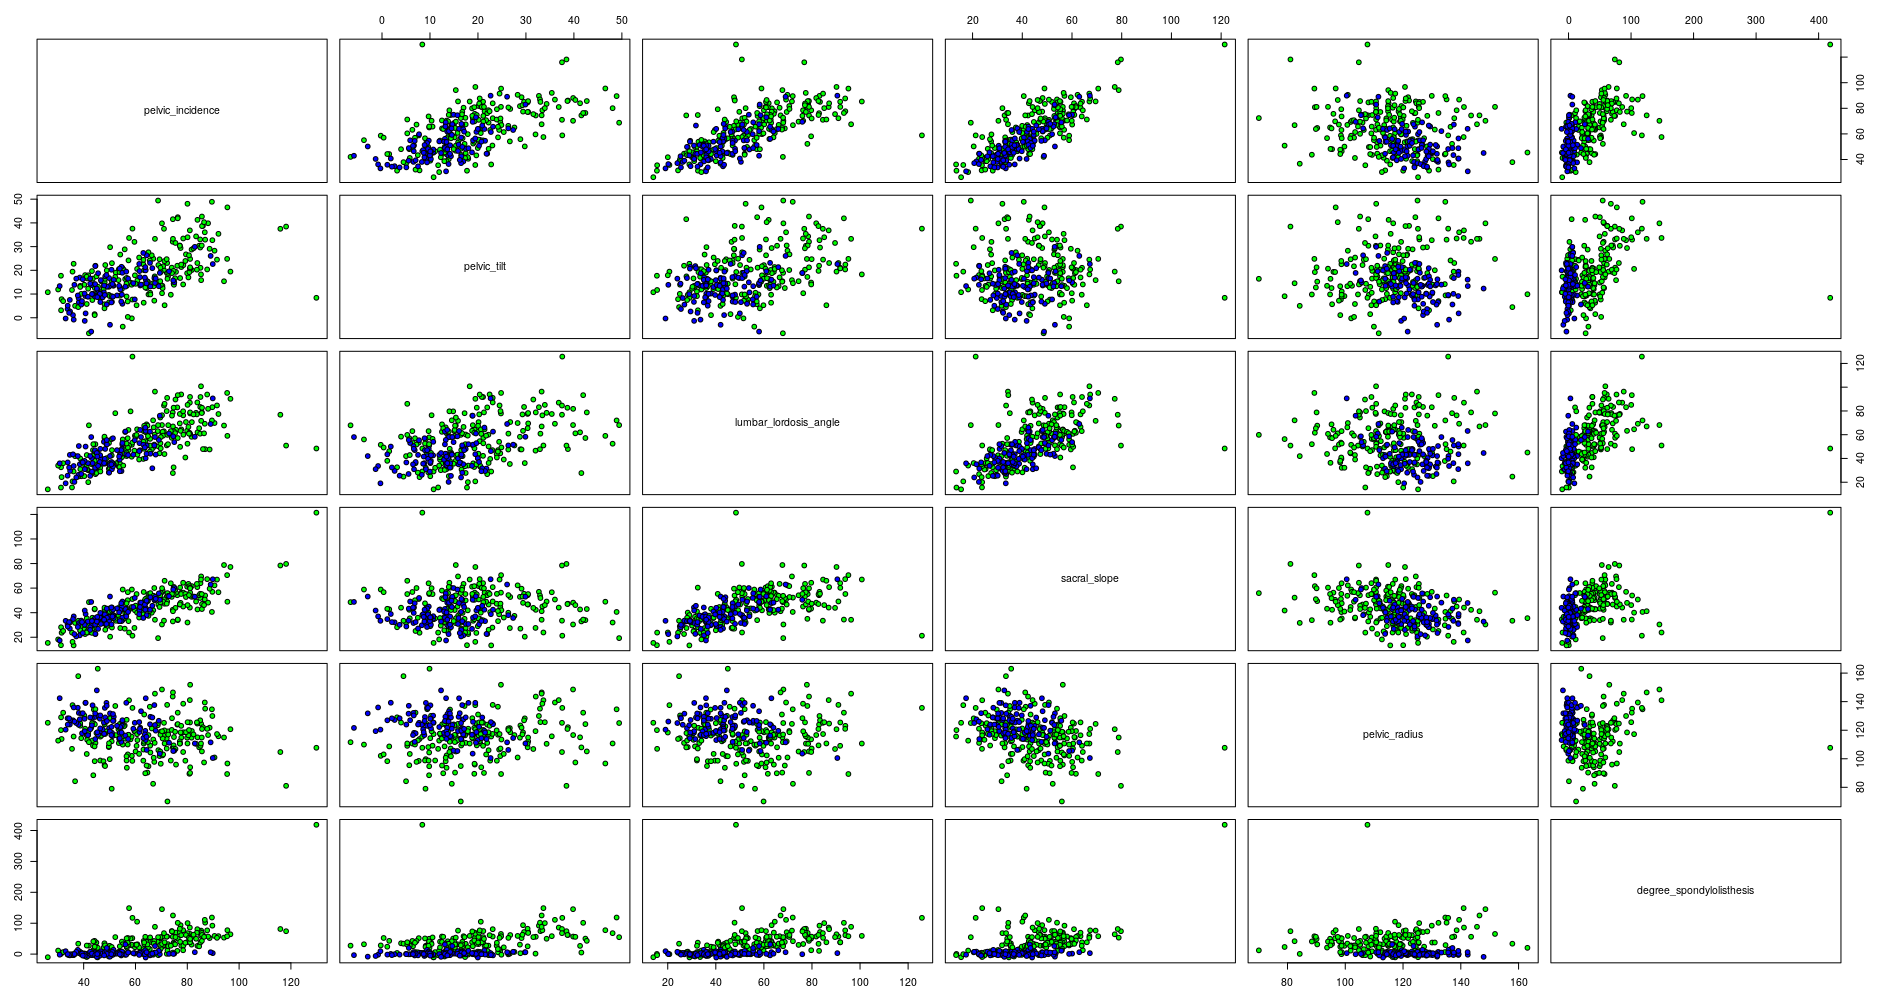
\includegraphics[width=\linewidth]{FeatureScatterPlot.png}
  \caption{Feature Scatter Plot}
  \label{fig:FeatureScatterPlot}
\end{figure}

\section{c.}

Given the values from section a and the scatter plot from section b we can see that the two classes are seperatated well by there values. For example if we pick two classes, pelvic\_radius and degree\_spondylolisthesis, we can compare the values and see how well they are seperated. If we also take into account the scatter plot from Figure \ref{fig:FeatureScatterPlot} we can see that abnormal classes have a larger value with respect of degree\_spondylolisthesis then the normal class.

\chapter{Section 2}

\section{a.}

Generating 100 3-dimensional vectors from a normal disribution with a mean vector as [1 2 1] and a 3x3 covariance matrix as [4  0.8 -0.3; 0.8 2 0.6; -0.3 0.6 5]

\begin{verbatim}
  mean <- c(1,2,1)
  cov <- matrix(c(4, 0.8, -0.3, 0.8, 2, 0.6, -0.3, 0.6, 5), 3,3)
  mvnd <- MASS\dotsmvrnorm(n = 100, mean, cov)
\end{verbatim}

\[
  cov=
  \begin{bmatrix}
    4 & 0.8 & -0.3 \\
    0.8 & 2 & 0.6 \\
    -0.3 & 0.6 & 5
  \end{bmatrix}
\]

\section{b.}

\section{c.}

\chapter{Section 3}

\chapter{Section 4}

\chapter{Section 5}

\end{document}
